\documentclass[confidential]{../../../classes/nervtech-engdoc}

\nervsetup{
  company={NervTech},
  project={Integrated Robotic Actuator},
  document={Integrated Robotic Actuator Technical Design Document},
  subtitle={Electromechanical architecture, control design, verification, and integration plan},
  docid={NT-N-MH-001},
  revision={A},
  status={Draft for Design Review},
  author={NervTech Engineering},
  owner={Robotics Systems Engineering},
  approver={Project Lead},
  date={2026-06-25},
  keywords={robotic actuator, BLDC, embedded control, torque sensing, mechatronics},
  abstract={This document details the design development of the Node actuator mechanical housing, integrated with the cycloidal reducer, based on requirements from NT-N-OVR-000, and research findings from NT-N-MH-000 and NT-N-CR-000. It includes derivation of design constraint regions based on requirements, and the final design solution with justification.},
}

\begin{document}
\maketitle
\tableofcontents
\newpage

\begin{revisionhistory}
  \revisionrow{A}{2026-06-25}{NervTech Engineering}{Initial technical document class demonstration.}
\end{revisionhistory}

\section{System Overview}
\systemsummary
{Adhesive bonded stator and rotor assembly with integrated cycloidal reducer and space for embedded control electronics.}
{Integrated PCB for FOC control, communication and power supply via USB-C or Molex.}
{Hall effect sensors for rotor position and speed feedback, with additional quadrature encoder for higher resolution.}
{Low reduction ratio for high backdrivability, and vibration compensation in cycloidal drive for less transfer to fixture.}

\section{Requirements}
There are several goals for Node that drive the requirements and design of the actuator.

\subsection{NT-N-G1}
From NT-N-OVR-000, NT-N-G1 has the following goal and success criteria:
\begin{quote}
  Goal: "The actuator should provide high precision torque and position control in high motion frequency applications."
  \\
  Success Criteria: "The actuator should be able to move standard payloads up to 20kgs at frequencies comparable to human motion."
\end{quote}
The components chosen must be able to account for failure modes induced by the stresses produced by the output load of up to 200N, applied at lever arms up to 0.25m, at frequency bandwiths up to 20Hz.
This interpretation of "frequencies comparable to human motion" is derived from \cite{HumanFrequencies}, which shows that human motion is typically in the range of 0.5Hz to 20Hz, however extended use of the upper limit is rarely reached.
The lever arm of 0.25m is derived from the half length of a human arm, which is approximately 0.6m, with the 200N payload derived from the weight of a 20kg object, which would be approximately 196N.
\\\\
The cycloidal speed reducer has inherent vibration characteristics, which must be accounted for in the design of the housing to ensure that the vibrations are not transferred to the fixture.
Since the cycloidal speed reducer also has inherent hertzian contact stresses, the housing must be able to withstand these stresses without failure.
\\\\
For the high accuracy and precision postional requirement, the overall backlash in the system should be kept to a maximum of 4 arcminutes, which would give a maximum positional error of 0.2525mm at a 0.25m lever arm, which is acceptable for the intended applications of the actuator.
\\\\
Torque ripple must also be kept to a minimum to meet the high accuracy and precision torque requirement, which is defined as a maximum of 0.5\% of the rated torque, which is 0.25Nm for the actuator.

\subsection{NT-N-G2}
From NT-N-OVR-000, NT-N-G2 has the following goal and success criteria:
\begin{quote}
  Goal: "The actuator should be reusable and easily integratable into a variety of frames for robotic systems."
  \\
  Success Criteria: "The actuator should be able to be mounted and dismounted with conventional tools from any of the standard NervTech linkages and/or frames."
\end{quote}
The housing should be able to be mounted via standardised metric machine screws, with the fasteners being able to be tightened with a standard hex key or torx key.
The fasteners must also be able to withstand the maximum torque applied to the actuator, which is 50Nm, without loosening or failing.
\\\\
The output flange must have the same mounting pattern as the mounting base, as this pattern will provide the basis for all future linkages and actuators in the Node family of products, and will allow for easy integration of the actuator into a variety of frames for robotic systems.
\subsection{NT-N-G7}
From NT-N-OVR-000, NT-N-G7 has the following goal and success criteria:
\begin{quote}
  Goal: "The actuator should be durable and reliable for long term use."
  \\
  Success Criteria: "The actuator should be able to operate for at least 10,000 hours of continuous operation without failure, and should be able to withstand standard industrial environmental conditions including dust and high moisture."
\end{quote}
The housing will be exposed to large temperature variations from stator heating, and as such it must be able to manage this heat long term to prevent failure.
The housing will also be highly vulnerable to failure from metallic dust and contaminats unless sealed to an appropriate IP rating, which will be determined based on the final design solution.
This may prevent a hollow shaft design, as this would require a large opening in the housing to allow for the shaft to pass through, which would compromise the sealing of the housing.
\\\\
Since cycloidal speed reducers have inherent hertzian contact stresses, the material selection for the cycloidal plates and rollers must be appropriate to prevent failure from these stresses, and the housing must be able to withstand the forces produced by these stresses without failure (including increase in backlash and torque ripple over time).
Cycloidal reducer bearings must also be chosen to withstand the forces produced by the output load at the maximum frequency of 20Hz, and the housing must be able to withstand the forces produced by these bearings without failure.

\begin{requirementstable}

  \reqrow
  {NT-N-IRQ1}
  {Performance}
  {The actuator shall withstand an output load of up to 200N applied at a lever arm of up to 0.25m at motion frequencies up to 20Hz without mechanical failure, including creep, plastic deformation, and fatigue.}
  {NT-N-G1}
  {Structural analysis and dynamic load test}

  \reqrow
  {NT-N-IRQ2}
  {Vibration}
  {The actuator housing shall limit the transfer of vibration generated by the cycloidal speed reducer to the external fixture.}
  {NT-N-G1}
  {Vibration test; acceptance criterion TBD}

  \reqrow
  {NT-N-IRQ3}
  {Structural}
  {The actuator housing shall withstand the reaction forces generated by Hertzian contact within the cycloidal speed reducer without structural failure.}
  {NT-N-G1}
  {Stress analysis and load test}

  \reqrow
  {NT-N-IRQ4}
  {Precision}
  {The total mechanical backlash of the actuator shall not exceed 4 arcminutes.}
  {NT-N-G1}
  {Backlash measurement test}

  \reqrow
  {NT-N-IRQ5}
  {Precision}
  {The actuator torque ripple shall not exceed 0.5\% of rated torque, corresponding to 0.25Nm at the 50Nm rated torque.}
  {NT-N-G1}
  {Torque ripple measurement}

  \reqrow
  {NT-N-IRQ6}
  {Interface}
  {The actuator housing shall be mountable and removable using standard metric machine screws tightened using conventional hex or Torx tools.}
  {NT-N-G2}
  {Inspection and assembly test}

  \reqrow
  {NT-N-IRQ7}
  {Structural}
  {The actuator mounting fasteners shall withstand the maximum actuator torque of 50Nm without loosening or mechanical failure.}
  {NT-N-G2}
  {Fastener analysis and proof-load test}

  \reqrow
  {NT-N-IRQ8}
  {Interface}
  {The actuator output flange shall use the same mounting pattern as the actuator mounting base.}
  {NT-N-G2}
  {Dimensional inspection}

  \reqrow
  {NT-N-IRQ9}
  {Reliability}
  {The actuator shall be capable of at least 10,000 hours of continuous operation without failure.}
  {NT-N-G7}
  {Reliability analysis and endurance testing}

  \reqrow
  {NT-N-IRQ10}
  {Environmental}
  {The actuator housing shall protect internal components from dust and high-moisture industrial environments using an appropriate enclosure sealing level.}
  {NT-N-G7}
  {IP environmental test; required rating TBD}

\end{requirementstable}

\begin{requirementstable}

  \reqrow
  {NT-N-IRQ11}
  {Thermal}
  {The actuator housing shall manage heat generated by the stator during continuous operation such that thermal loading does not cause component or housing failure.}
  {NT-N-G7}
  {Thermal analysis and continuous-load thermal test}

  \reqrow
  {NT-N-IRQ12}
  {Durability}
  {The cycloidal plates and roller pins shall use materials capable of withstanding the expected Hertzian contact stresses over the required operating life without failure.}
  {NT-N-G7}
  {Hertzian stress analysis and material verification}

  \reqrow
  {NT-N-IRQ13}
  {Durability}
  {The cycloidal reducer bearings shall withstand the forces generated by the maximum specified output load at operating frequencies up to 20Hz without failure.}
  {NT-N-G7}
  {Bearing load and life analysis}

  \reqrow
  {NT-N-IRQ14}
  {Structural}
  {The actuator housing shall withstand the reaction forces transmitted by the cycloidal reducer bearings throughout the required operating life without structural failure.}
  {NT-N-G7}
  {Structural analysis and endurance test}

  \reqrow
  {NT-N-IRQ15}
  {Durability}
  {Wear and deformation of the cycloidal reducer and its supporting structure shall not cause backlash or torque ripple to exceed their specified limits over the required operating life.}
  {NT-N-G7}
  {Endurance test with pre- and post-test backlash and torque-ripple measurement}

\end{requirementstable}
\newpage
\section{Design}
\subsection{Rotor Cup Design}
\subsubsection{Bond Line Specifications}
The rotor cup design must be mounted to the rotor such that the rotor cup does not slip or rotate relative to the rotor during operation, as this would cause a loss of torque transmission and potentially damage the actuator (NT-N-IRQ1).
From research done in NT-N-MH-000, adhesive bonding using retaining compounds will be the preferred method to accomplish this goal. The following retaining compound has been identified as a suitable candidate for this application:
\begin{figure}[H]
  \centering
  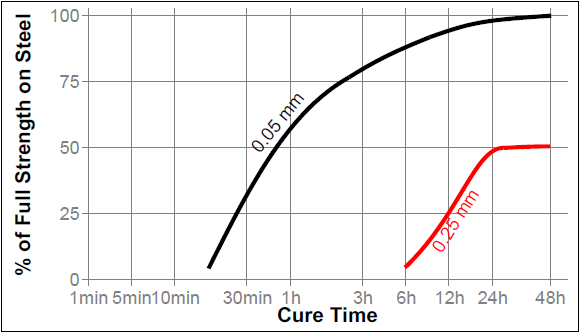
\includegraphics[width=0.7\textwidth]{figures/BondLinevsCureStrength.png}
  \caption{Bond Line Thickness vs. Cure Strength for Retaining Compounds}
  \label{fig:Loctite640BondLineStrength}
\end{figure}
From the data in Figure \ref{fig:Loctite640BondLineStrength}, it can be seen that the bond line thickness must be kept to a minimum of 0.05mm, and a maximum of of 0.25mm, to ensure the bond line strength is between 50\% and 100\%, assuming steel on steel bonding.
The closer the bond line thickness is to 0.05mm, the higher the bond line strength will be, and the more torque can be transmitted through the bond line without failure.
From the WK8115 datasheet specification (see NT-N-MH-000), the tolerance of the rotor back iron outer diameter is $\pm$0.1mm, which already exceeds the minimum bond line thickness of 0.05mm.
\subsubsection{Rotor Cup Tolerances}
The rotor cup tolerance must be within $\pm$0.025mm to ensure that the bond line thickness has a maximum thickness of 0.25mm, which in the worst case reduces the bond line strength to 50\% of the maximum strength on steel.
This is suitable for the application, as the maximum torque transmitted through the bond line is 5.83Nm from NT-N-MH-000, and the breakaway torque at 50\% is at a minimum 10Nm after curing.
\\\\
It must also be located such that its central axis is aligned with the rotor axis, as any misalignment would cause uneven air gaps (see NT-N-MH-000 for preliminary research), leading to torque ripple and potential damage to the actuator (NT-N-IRQ1) (NT-N-IRQ5).
Slots for locating pins can be machined onto the backiron at 180° separation, and corresponding slots can be machined onto the rotor cup to accommodate these pins (NT-N-IRQ1) (NT-N-IRQ5).
\subsubsection{Rotor Cup Cycloidal Integration}
From the research done in NT-N-CR-000, to integrate an epitrochoidal-pinwheel speed reducer into the actuator (NT-N-IRQ1), 2 epitrochoidal profiles in 180° phase separation must be machined and placed on cranks, also with 180° phase separation.
The 2 epitrochoidal profiles reduce the vibration from the eccentric orbit of one profile (NT-N-IRQ2).
To make the stackup of rotor cup - eccentric shaft - bearing - reducer as compact as possible, the bearings used must have minimal thickness while being able to withstand the overturning moment forces of the cycloidal output, and the radial forces from their respective eccentric orbits (NT-N-IRQ13).
The cycloidal discs must furthermore be machined of materials that minimise thickness while withstanding all hertzian contact stresses, and output load stresses (NT-N-IRQ12).
\subsubsection{Rotor Cup Force Analysis}
According to NT-N-IRQ1, the actuator should be able to apply 200Nm at a lever arm of 0.25m, up to 50Hz.
Resisting axial forces as a result of moving loads is not mentioned in the requirements and is therefore not considered in the stress analysis.
Static axial forces will, however, be considered as the actuator may be mounted in a variety of configurations, which may include resistance of a payload's weight when mounted parallel to the ground.
\\\\
To make a simplified model of the most basic load the actuator will have to carry, the following free body diagram was created, in the plane normal to the rotational axis fo the actuator (note the rectangular beam is represenational, and may have a more complex geometry and mass distribution):
\begin{figure}[H]
  \centering
  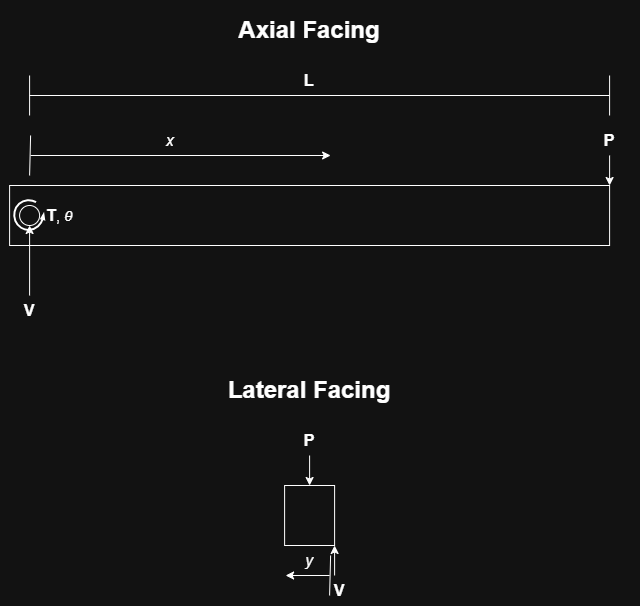
\includegraphics[width=0.7\textwidth]{figures/FreeBodyDiagrams_Beam.png}
  \caption{Simplified Load FBD}
  \label{fig:SimplifiedLoadFBD}
\end{figure}
The parameter of interest is $\theta$, which denotes the angular displacement of the actuator.
The output torque of the actuator is denoted as $T$, and the radial reaction force of the bearing is denoted as $V$.
Using the free body diagram, we can find the equation of motion of the actuator (disregarding its internal dynamics at this stage) and the statics of the radial load on the bearings.
\[
\begin{aligned}
  J\ddot{\theta}&=T - \int_{0}^{L}9.8\cdot m(x) x\cos{\theta}dx - PL
  \\
  0 &= V - P - 9.81M
\end{aligned}
\]
$m(x)$ is the function of linkage mass at distance $x$, and $M$ is the total mass of the linkage.
The mass moment of inertia $J$, is a function of the properties of the beam, and may be defined as follows:
\[
\begin{aligned}
  J = \int r_{\perp}^{2}\,dm
\end{aligned}
\]
We consider the idealised worst case, where the mass of the linkage is concentrated at its very end, and then compute the mass moment of inertia as well as the other mass dependent terms. According to NT-N-IRQ1, the mass would be 20kgs:
\[
\begin{aligned}
  J &= 20L^2
  \\
  20L^2\ddot{\theta} &=T - 20 \cdot 9.8 \cdot \cos\theta L - PL
  \\
  T &= 20L^2\ddot{\theta} + 20 \cdot 9.8 \cdot \cos\theta L + PL
  \\
  T &= 20L^2\ddot{\theta} + 20 \cdot 9.8 \cdot \cos\theta L + PL
\end{aligned}
\]
With $L$ being 0.25 metres, and assuming the very limit of capability being when acceleration is 0, the equation simplifies to:
\[
\begin{aligned}
  T = 49\cos\theta + 0.25P
\end{aligned}
\]
Since NT-N-IRQ1 requires only a 20kg payload to be carried in frequencies comparable to human motion, we can assume that in the worst case, with $\cos \theta$ being 1, we will not be able to apply any external, torque-generating forces, represented by $P$.
However, as $\cos \theta$ goes to 0, these external forces may increase up to 196N to match the force generated by a 20kg payload in the worst case.
\\\\
Standard integrated actuators output generated power through a flange, with the output payload being fastened to the flange via machine screws.
The force and stress analysis done on the flange will be used to choose the correct output transmission bearing.
\\\\
From the analysis already done in the Axial Facing Plane, the radial load on the bearing will be at a maximum 196N.
In the bottom of Figure~\ref{fig:SimplifiedLoadFBD} the Lateral Facing free body diagram is represented.
In the simplified version of the free body diagram, if the beam is subject to the entire weight of the load (which is at a maximum 196N derived from NT-N-IRQ1) in the axial direction, then the output bearing must resist axial laods of up to 196N.
\\\\
As $P$ is applied with some offset y to the fastened plane on the right, there will be a moment created on the output bearing:
\[
M = P \cdot y
\]
As an assumption, the width of the lever arm described in NT-N-IRQ1 will not exceed its length, and is therefore capped at 0.25m (even this case is unrealistic).
Therefore, the moment will be, at worst, as follows:
\[
\begin{aligned}
  M &= 196 \cdot 0.25
  M &= 48Nm
\end{aligned}
\]
Finally, the output speed is required for finalising output bearing choice.
NT-N-IRQ1 dictates that the payload will move at motion frequencies of 20Hz, and it is assumed that the angular displacement of one cycle is at a maximum half a revolution.
Thus, the calculation for angular velocity is as follows:
\[
  \omega = 20\pi \ rad\cdot s^{-1}
\]
The bearing must be able to resist these loads at 600RPM for 10,000 hours without failure (NT-N-IRQ1, NT-N-IRQ9, NT-N-IRQ13)
Since the actuator should also be sealed from dust and high moisture (NT-N-IRQ10), the bearing should be sealed.
A table of the bearing requirements is as follows:
\begin{itemize}
  \item Must last for 10,000 hours without failing.
  \item Must resist 196N of axial force.
  \item Must resist 196N of radial force.
  \item Must resist 49Nm of overturning moment force.
  \item Must operate at 500 RPM.
\end{itemize}


\begin{thebibliography}{9}

  \bibitem{HumanFrequencies}
  Piyarathna, Iresha \& Thabet, Ahmed \& Ucgul, Mustafa \& Lemckert, Charles \& Lim, Yee Yan \& Tang, Zi Sheng. (2023). Linear Segmented Arc-Shaped Piezoelectric Branch Beam Energy Harvester for Ultra-Low Frequency Vibrations. Sensors. 23. 10.3390/s23115257.

\end{thebibliography}

\end{document}
